% Charlotte Geiger - Manuel Lippert - Leonard Schatt
% Physikalisches Praktikum

% Teilauswertung 2

\section{Nutation}

Die Nutation ist eine zusätzliche Komponente zur Präzession. Bei genauer Beobachtung des Kreisels kann man neben der Präzessionsbewegung erkennen, dass die Kreiselachse nicht komplett ruhig um die Senkrechte läuft, sondern viel mehr kleine Rotationen auf der Bahn der Präzession vollführt. Das ist das Phänomen der Nutation.\\
Um diese Nutation des Kreisels zu untersuchen, bestimmt man die Nutationsfrequenz des momentfreien Kreisels als Funktion von $\omega_3$. Damit es gut darzustellen und auszuwerten ist, betrachtet man $w_3$ im Bezug zu dem Quotienten $\frac{w_n}{w_3}$, wobei dieser vortan als $\omega_N$ bezeichnet wird. \\
Um die Frequenz in die Winkelgeschwindigkeit umzurechnen, muss man die Frequenz mit $2\pi$ multiplizieren $(w =2\pi\cdot f)$.\\
Der Fehler des Stroboskops wird abgeschätzt mit $u_{f_3}=0.25$ Hz, da der Ablesefehler für die verwendete Messmethode zu optimistisch ist. 
Auch bei der Zeitmessung muss der Fehler mitbetrachtet werden, dieser wird abgeschätzt mit dem Ablesefehler auf $u_a=u_t=0.01~s$. Wobei dabei der Mittelwert der Zeiten aus den beiden Messreihen gebildet und dieser durch 10 geteilt (wegen 10 Umdrehungen) wird, um die Rotationsdauer $T_n$ zu erhalten. Daraus folgen die Formeln mit Fehlerfortpflanzungsgesetz:
\begin{gather}
    \omega_3^i=2\pi\cdot f_3^i  \tab \omega_n^i = \frac{2\pi}{T_n^i}\\
    t_n^i = \frac{t_{n_1}^i+t_{n_2}^i}{2}\tab u_{t_n} = \frac{u_t}{\sqrt{2}} \tab T_n^i=\frac{t_n^i}{10} \tab u_{T_n} = \frac{u_{t_n}}{\sqrt{10}}\\[0.3mm]
    \omega_N^i=\frac{\omega_n^i}{\omega_3^i} = \frac{1}{T_n^i f_3^i} 
    \tab u_{\omega_N^i} = \sqrt{{(\frac{u_{T_n}}{{T_n^i}^2f_3^i})}^2+{(\frac{u_{f_3}}{T_n^i{f_3^i}^2})}^2} 
\end{gather}
Um das Verhältnis von $\omega_3$ im Bezug zu $\omega_N$ tabellarisch aufzutragen, muss man auf das Vorzeichen achten. Aus den Eulerschen Gleichungen für den momentfreien, symmetrischen Kreisel wurde folgendes im Skript angegeben:
\begin{align}
    \omega_N^i = \frac{J_3 - J_1}{J_1} = \text{konstant}
\end{align}
Da wir aber nur noch einen symmetrischen Kreisel mit $J_1 = J_2$ und $J_3<J_1$ betrachten, ist das konstante Verhältnis negativ, was mit einem - Zeichen bei $\omega_N$ verdeutlicht wird. 
\newpage
\begin{center}
    \captionof{table}{Nutationswerte}
    \begin{tabular}{gcccccccc}
        \rowcolor[rgb]{ .741,  .843,  .933}{} &     $t_n~[s]$ &   $u_{t_n}~[s]$ &     $T_n~[s]$ &   $u_{T_n}~[s]$ &      $\omega_3~[\frac{1}{s}]$ &    $\omega_n~[\frac{1}{s}]$ &      $\omega_N$ &    $u_{\omega_N}$ \\
        1  &  61.33 &  0.007 &  6.133 &  0.002 &   62.83 &  1.02 & -0.0163 &  0.0004 \\
        2  &  59.17 &  0.007 &  5.917 &  0.002 &   65.97 &  1.06 & -0.0161 &  0.0004 \\
        3  &  58.32 &  0.007 &  5.832 &  0.002 &   69.12 &  1.08 & -0.0156 &  0.0004 \\
        4  &  51.33 &  0.007 &  5.133 &  0.002 &   75.40 &  1.22 & -0.0162 &  0.0003 \\
        5  &  49.25 &  0.007 &  4.925 &  0.002 &   81.68 &  1.28 & -0.0156 &  0.0003 \\
        6  &  45.16 &  0.007 &  4.516 &  0.002 &   87.96 &  1.39 & -0.0158 &  0.0003 \\
        7  &  40.66 &  0.007 &  4.066 &  0.002 &   94.25 &  1.55 & -0.0164 &  0.0003 \\
        8  &  37.88 &  0.007 &  3.788 &  0.002 &  100.53 &  1.66 & -0.0165 &  0.0003 \\
        9  &  36.01 &  0.007 &  3.601 &  0.002 &  106.81 &  1.74 & -0.0163 &  0.0002 \\
        10 &  34.45 &  0.007 &  3.445 &  0.002 &  113.10 &  1.82 & -0.0161 &  0.0002 \\
        11 &  32.96 &  0.007 &  3.296 &  0.002 &  119.38 &  1.91 & -0.0160 &  0.0002 \\
        12 &  30.97 &  0.007 &  3.097 &  0.002 &  125.66 &  2.03 & -0.0161 &  0.0002 \\
    \end{tabular}
\end{center}
\begin{figure}[ht]
    \centering
    \caption{$w_N$ Histogramm}
    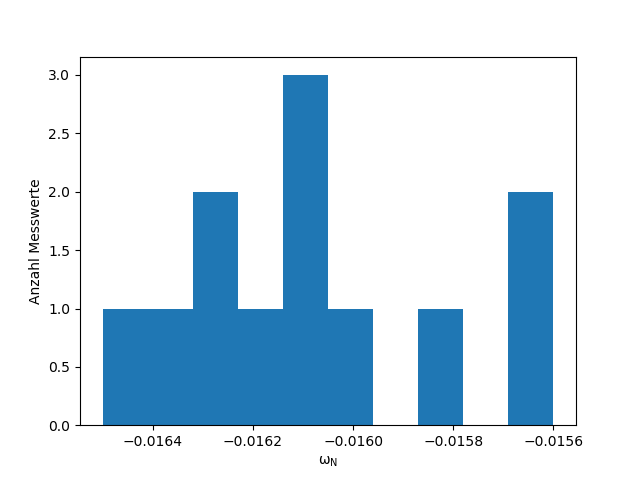
\includegraphics[scale=0.6]{6_2-Hist.png}
\end{figure}
Nun wird die Konstante durch den Mittelwert der berechneten Verhältnisse berechnet.
\begin{align}   
    \overline{\omega_N} = \frac{1}{M}\sum_{i=1}^{M}\omega_N^i \tab u_{\overline{\omega_N}}= \frac{1}{M}\sqrt{\sum_{i=1}^{M}s_{\omega_N^i}^2} \tab M:\text{Anzahl der Werte}
\end{align}
Da aber die Werte von $\omega_N$ sehr nah beianderliegen wird der Fehler des Mittelwerts vernachlässigt und der Fehler von $\overline{\omega_N}$ als Mittelwert der Fehler von $\omega_N$ abgeschätzt.
\begin{align*}
    \Rightarrow\boxed{\overline{\omega_N}=(-0.0161\pm0.0003)}
\end{align*}
\newpage
\begin{figure}[ht]
    \centering
    \caption{$\omega_3-\omega_N$ Diagramm}
    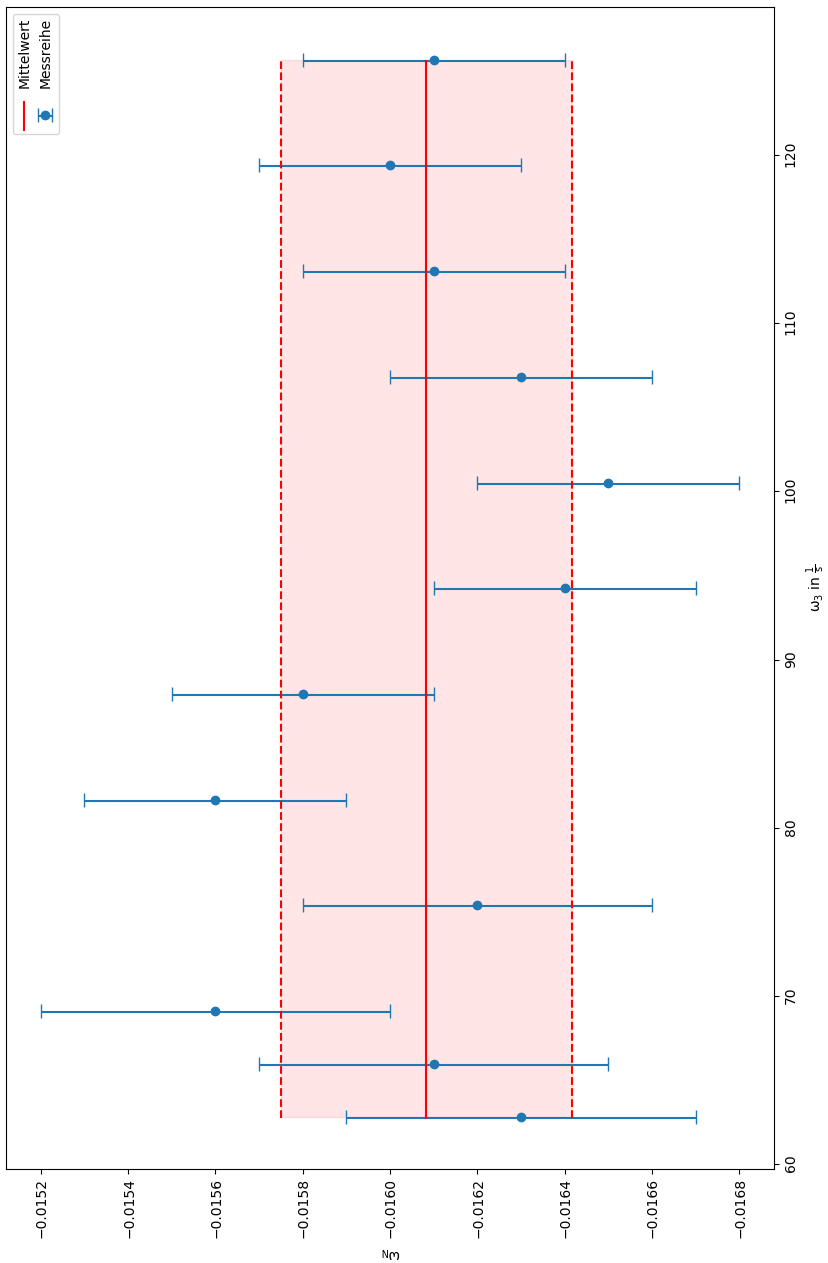
\includegraphics[scale=0.6]{6_2-Nutation.png}
\end{figure}